\documentclass[a4paper,12pt]{article}
\usepackage[utf8]{inputenc}
\usepackage[brazil]{babel}
\usepackage{fullpage}
\usepackage{times}
\usepackage{setspace}
\usepackage{indentfirst}
\usepackage[pdftex]{graphicx}
\usepackage{subfigure}
\usepackage{url}
\usepackage{pdfpages}

\usepackage[cmex10]{amsmath}
\usepackage{hyperref}
\usepackage{cite}

\title{\hrule\vspace{1pt}\hrule\vspace{25pt}}
\author{\LARGE \bf Lucio Mitsuru Seki}

\date{\Large \bf Janeiro de 2012 \vspace{25pt}\hrule\vspace{1pt}\hrule}

\renewcommand{\floatpagefraction}{0.9}
\renewcommand{\textfraction}{0}
\setcounter{bottomnumber}{4}

\graphicspath{{figuras/}}
\usepackage{color}
\usepackage{listings}
\lstset{
	language=C,
	basicstyle=\footnotesize,
	numbers=left,
	numberstyle=\footnotesize,
	stepnumber=1,
	numbersep=5pt,
	backgroundcolor=\color{white},
	showspaces=false,
	showstringspaces=false,
	showtabs=false,
	frame=single,
	tabsize=2,
	captionpos=b,
	breaklines=true,
	breakatwhitespace=false
}

\begin{document}
\pagestyle{empty}
\onehalfspacing
\begin{center}
{\Large \bf Universidade Federal de São Carlos campus Sorocaba}\\[15pt]
{\Large Bacharelado em Ciência da Computação}\\[15pt]
{\Large Multimídia Computacional\\ Professor Murillo Rodrigo Petrucelli Homem}
\vfill
\vfill
{\Large Técnica de compressão de ADPCM para armazenamento de áudio}
\vfill
\vfill

{\Large Lucio Mitsuru Seki}\\
\bigskip
{Sorocaba/2013}
\end{center}

\newpage

\section{Introdução}

\paragraph{}
A armazenagem de um sinal de áudio na forma digital possui várias vantagens, facilitando a aplicaçao de filtros, a transmissão entre dispositivos, a reprodução e a organização; diminuindo a incidência de ruídos, entre outras. No entanto, precisamos comprimí-lo para viabilizar o seu armazenamento e transmissão.

\paragraph{}
Uma das abordagens simples de compressão de áudio é ADPCM, uma técnica baseada na redundância no sinal original. Neste artigo descrevo a técnica de compressão ADPCM, e mostro uma implementação simplificada de um codec ADPCM.

\section{Definições}

\paragraph{}
A técnica de compressão \textit{Adaptive Differential PCM} - ADPCM se baseia na técnica de armazenamento \textit{Pulse-code Modulation} - PCM, e também na abordagem \textit{Differential PCM} - DPCM de compressão de áudio. Descrevo abaixo estes conceitos.

\subsection{Codec}

\paragraph{}
Um \textit{Coder-decoder} - codec é um software com um par de algoritmos para codificar e decodificar um sinal multimídia, seja de áudio, de imagem ou de vídeo. No contexto atual, a necessidade de codificação sempre está atrelada à necessidade de compressão do arquivo de multimídia, devido a quantidade elevada de memória necessária para armazenar o sinal, e de banda de transmissão para enviar o mesmo de um dispositivo para outro.

\paragraph{}
Um algoritmo de compressão pode ser com perda ou sem perda. Na abordagem com perda, tiramos proveito das características psicofísicas do Homem para reconhecer e interpretar o sinal, e na abordagem sem perda, a característica redundante do sinal.

\paragraph{}
Há codecs que usam vários algoritmos de compressão, até mesmo combinando os com perda e os sem perda. Dependendo da aplicação, pode melhorar a taxa de compressão, o tempo de compressão ou minimizar a perda.

\subsubsection{Algoritmo de compressão com perda}
\paragraph{}
Quando o Homem não percebe a redução na qualidade e/ou na fidelidade do sinal, não há necessidade de armazenar este excesso de informações imperceptíveis. Então podemos aplicar um algoritmo de compressão com perda sobre o sinal.  A redução de qualidade causada pela compressão pode até ser perceptível, mas pode ser tolerável dependendo da aplicação.

\paragraph{}
O algoritmo costuma ser rápido, pois pelos estudos prévios de espcialistas sobre a percepção humana, já conhecemos os vieses a considerar para eliminar informações. Basta aplicar o algoritmo em tempo linear conforme percorre o arquivo.

\paragraph{}
Dizemos que o algoritmo é com perda, pois o sinal pode ser interpolado de alguma forma, mas é impossível recuperar o sinal original através da descompressão.

\subsubsection{Algortimo de compressão sem perda}

\paragraph{}
Em muitos casos, o sinal possui algum tipo de redundância. Numa imagem pode ser pixels adjacentes com cores similares. Num sinal de áudio pode ser uma diferença reduzida no valor das amostras vizinhas. Neste caso podemos aplicar um algoritmo de compressão sem perda.

\paragraph{}
Este tipo de algoritmo costuma ser mais complexo do que os algoritmos com perda, pois considera alguma característica redundante entre as amostras do sinal, tendo que realizar várias comparações. Os algoritmos de compressão baseada na redundância também são computacionalmente caros. Em compensação, o sinal recuperado é idêntico ao original.

\subsection{WAVE PCM}

\paragraph{}
A PCM é uma representação digital de um sinal de áudio. Suas origens se dão desde os meados do século XIX, no campo da telegrafia, mas a codificação de áudio foi iniciado durante a segunda guerra mundial.

\paragraph{}
A Bell Labs iniciou o seu aperfeiçoamento nos anos 40. A técnica é implementada num dispositivo conversor analógico-digital, que quantiza as amostras do sinal analógico atribuindo um valor discreto proporcional a cada amostra. Esta sequência de valores é armazenada para reprodução posterior.

\paragraph{}
O \textit{Waveform Audio File Format} - WAVE é um padrão de armazenamento de arquivos de áudio, baseado no modelo de \textit{container} \textit{Resource Interchange File Format} - RIFF, desenvolvido pela Microsoft e IBM em 1991\cite{Microsoft-IBM-1991}.

\begin{figure}[!htb]
	\centering
	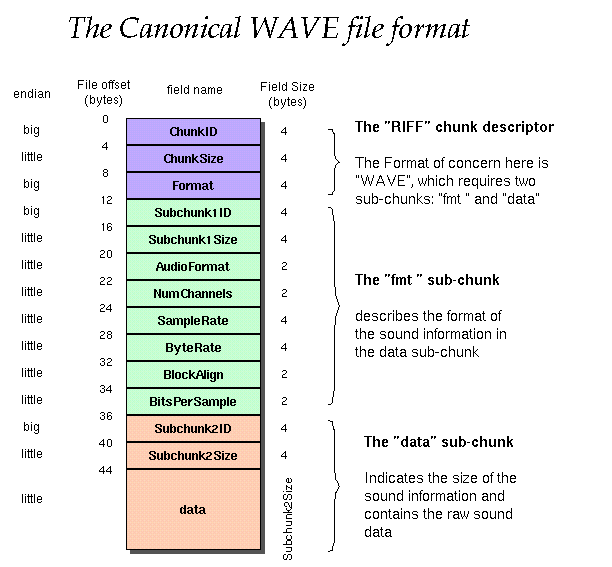
\includegraphics[width=\paperwidth/2]{wav-sound-format.png}
	\caption{Cabeçalho WAVE}
	\label{fig:wave-header}
\end{figure}

\begin{figure}[!htb]
	\centering
	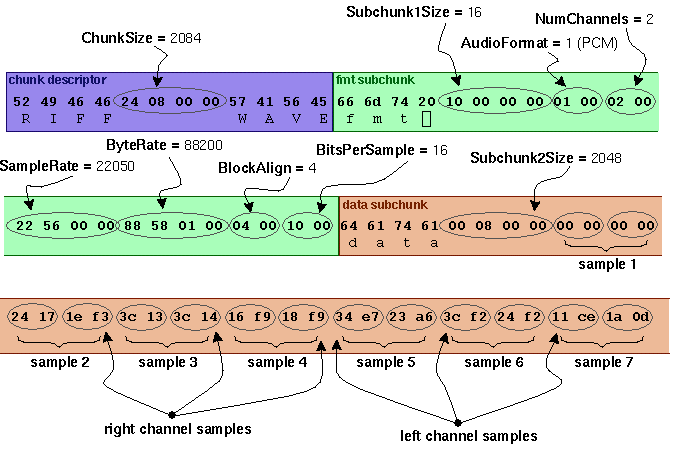
\includegraphics[width=\paperwidth/2]{wave-bytes.png}
	\caption{Exemplo de um arquivo WAVE}
	\label{fig:wave-bytes}
\end{figure}

\paragraph{}
WAVE PCM é uma forma simples de armazenar um sinal de áudio. Consiste de um cabeçalho RIFF, e o conjunto de bytes representando o sinal de áudio propriamente dito, na representação por PCM. Um exemplo simples de arquivo WAVE PCM é ilustrado na figura ~\ref{fig:wave-bytes}.

\paragraph{}
O cabeçalho WAVE PCM está ilustrado na figura \ref{fig:wave-header} e implementado em C no código \ref{code:wave-header}

\paragraph{}
O cabeçalho WAVE armazena informações como o formato do arquivo, o método de compressão, número de canais, taxa de amostragem e tamanho do arquivo; dados importantes para a correta reprodução e codificação do áudio.

\paragraph{}
O armazenamneto no formato canônico (PCM) exige muito espaço em memória, e a sua transmissão exige uma banda bem larga, conforme a duração e a taxa de amostragem aumentar. Este problema ainda não é despresível com a tecnologia que temos hoje.

\subsection{DPCM}

\paragraph{}
A compressão do sinal de áudio foi proposta por um engenheiro da Bell Labs em 1950\cite{Cutler-1950}, numa época em que a capacidade dos dispositivos eletrônicos era bastante reduzida. A finalidade era de reduzir o tráfego de dados na rede de telefonia fixa. Havia a necessidade de executar o algoritmo em alguns milissegundos sobre pequenos trechos da fala, para que os usuários não percebessem o atraso causado pelo algoritmo.

\paragraph{}
No nosso contexto de compressão de arquivos de áudio para armazenamento, temos capacidade computacional milhões de vezes maior nos nossos computadores pessoais, e podemos executar o algoritmo sobre o arquivo todo para armazená-lo e descomprimí-lo posteriormente.

\paragraph{}
Este algoritmo de compressão foi criada pela observação da redundância no sinal de áudio. Os valores dos sinais quantizados costumam ser não muito distantes uns dos outros na sequência. Portanto, podemos armazenar a diferença de valor entre as amostras na sequência. Esta diferença costuma ser várias ordens de grandeza menores do que o valor de cada amostra e, portanto, podemos reduzir a quantidade de bits para representar cada amostra.

\paragraph{}
O algoritmo varre todo o arquivo e utiliza apenas a quantidade de bits necessária para representar a maior diferença entre as amostras na sequência. A diferença de uma amostra para a outra pode ser negativa, portanto utiliza-se um bit para representar o sinal do valor da diferença, em complemento de dois.

\subsection{ADPCM}

\paragraph{}
Esta técnica foi proposta em 1973 pela Bell Labs\cite{Cummiskey-Jayant-Flanagan-1973}, num cenário não muito diferente da proposição do DPCM.

\paragraph{}
A abordagem DPCM é simples, mas possui uma desvantagem por utilizar a quantidade de bits necessária para representar a maior diferença entre as amostras em sequência no arquivo todo.

\paragraph{}
Esta diferença pode ser minimizada ao dividir o arquivo em segmentos menores. Ao segmentar o arquivo, cada segmento passa a ter uma amostra chave, a partir da qual calculam-se as diferenças em sequência. Assim, cada segmento passa a ter a sua maior diferença, representando-a com uma determinada quantidade de bits.

\paragraph{}
Muitas vezes, esta abordagem reduz o tamanho total do arquivo, por considerar uma quantidade ótima local de bits em cada segmento, em vez de utilizar uma quantidade global de bits em todo o arquivo.

\paragraph{}
A segmentação do áudio pode ser feita seguindo diversos critérios. Uma abordagem da Interactive Multimedia Association - IMA é de consultar duas tabelas que, de acordo com o valor da amostra, indica a mudança no tamanho do segmento e/ou na quantidade de bits por amostra no segmento atual\cite{Pan-1993}.

\paragraph{}
Neste artigo fiz uma implementação mais simples, onde o WAVE original é segmentado em duzentas partes. Após processar as amostras num segmento, o algoritmo escolhe a próxima amostra como chave, a partir da qual calcula a diferença das amostras subsequentes, e assim repetidamente.
Não implementei a descompressão até o presente momento.

\section{Implementação}

\paragraph{}
Listei abaixo a implemntação em linguagem C de cada um dos conceitos descritos na seção anterior.

\paragraph{}
Cabeçalho WAVE PCM
\lstinputlisting[caption=wave\_header.h, label=code:wave-header]{wave_header.h}

\paragraph{}
Programa principal
\lstinputlisting[caption=main.c, label=code:main]{main.c}

\paragraph{}
Cabeçalho do Codec
\lstinputlisting[caption=adpcm\_codec.h, label=code:adpcm-codec-header]{adpcm_codec.h}

\paragraph{}
Funções do Codec
\lstinputlisting[caption=adpcm\_codec.c, label=code:adpcm-codec-body]{adpcm_codec.c}

\section{Conclusão}

\paragraph{}
Nesta abordagem, ao utilizar um arquivo de música de 1.130.624 bytes como entrada, resultou num arquivo de saída 848 bytes. Isto significa uma razão de compressão de 1333.28. Não foi conferido se a compressão está correta.
A maior dificuldade na execução do trabalho foi a de utilizar os operadores binários de shift, por falta de prática.

\begin{thebibliography}{}
	\bibitem{Microsoft-IBM-1991} MICROSOFT; IBM. Multimedia Programming Interface and Data Specifications 1.0. 1991.
	\bibitem{Cutler-1950} CUTLER, C.C., Differential Quantization of Communication Signals. United States patent 2605361. 1950 June 29.
	\bibitem{Cummiskey-Jayant-Flanagan-1973} CUMMISKEY, P.; JAYANT, N.S.; FLANAGAN, J.L. Adaptive Quantization in Differential PCM Coding of Speech. \textit{The Bell System Technical Journal}, v. 52, n. 7, p. 1105-1118, 1973.
	\bibitem{Pan-1993} PAN, D.Y. Digital Audio Compression. \textit{Digital Technical Journal}, v. 5, n. 2, p. 28-40, 1993.
\end{thebibliography}
\end{document}
